In this section, we introduce LP-RFFs, and present our theoretical results, which lower bound the probability that $D_{\lambda}(K,\tK) \leq \Delta$, where $\tK$ is the kernel approximation matrix corresponding to $m$ low-precision random Fourier features (LP-RFFs). This directly implies a bound on the generalization performance of LP-RFFs, using Proposition \ref{prop:avron}. We validate our theoretical results on a subset of the Census UCI dataset, showing that one can achieve lower relative spectral distance per bit by using LP-RFFs, relative to full-precision \Nystrom features or RFFs.  This is true even when we only consider the space occupied by the features themselves.

\subsection{Method details}
\label{subsec:method_details}
The core idea behind LP-RFFs is to use $b$ bits to store each RFF, instead of $32$ or $64$ bits. We implement this using a simple stochastic rounding scheme. Given that $z_i(x) = \sqrt{2/m}\cos(w_i^T x + a_i) \in [-\sqrt{2/m},\sqrt{2/m}]$, we can divide this interval into $2^b - 1$ sub-intervals of equal size. We then randomly round each feature $z_i(x)$ to either the top or bottom of the interval containing it, in such a way that the expected value is equal to $z_i(x)$. Defining $\delta_b^2 \defeq \frac{2}{(2^b-1)^2}$, the variance of this unbiased rounding scheme is at most $\delta_b^2/m$.  As a way to reduce the memory footprint during training even further, we leverage existing work on using circulant random matrices \citep{yu15} so that the RFF random projection matrix only occupies $32m$ space.

\subsection{Theoretical results}

We now lower bound the probably that $D_{\lambda}(K,\tK) \leq \Delta$, for the LP-RFF approximation $\tK$ using $m$ features and $b$ bits per feature.

\begin{theorem}
	\label{thm2}
	Let $\tK = (Z+C)(Z+C)^T$ be the LP-RFF approximation of a kernel matrix $K$, where $Z\in\RR^{n\times m}$ denotes the full precision RFF matrix, and $C$ denotes the quantization noise.  We assume $\expect{}{C_{ij}} = 0$ and $\var[C_{ij}] \leq \delta_b^2 \;\;\forall i,j$, where $b$ is the number of bits used per feature. Suppose that $\norm{K} \geq \lambda$ and $\delta^2_b \leq \lambda$. Then for any $\Delta \in \Big[\frac{3}{2}\sqrt{\frac{2n/\lambda}{m}} + \frac{2n/\lambda}{m} + \frac{3}{2}\frac{\delta^2_b}{\lambda}, \frac{1}{2} \Big]$,
	\begin{equation*}
	%(1 + \Delta)^{-1}(K + \lambda I_n) \preceq (Z + C) (Z + C)^\top + \lambda I_n \preceq (1 + \Delta)(K + \lambda I_n)
	\Prob\Big[D_{\lambda}(K,\tK) \leq \Delta\Big] \geq 1 - 16 \tr((K + \lambda I_n)^{-1} (K + \delta^2_b I_n)) \exp \left( -\frac{9m \big(\frac{2}{3}\Delta - \delta^2_b / \lambda\big)^2}{44n/\lambda} \right).
	\end{equation*}
	Thus if we use 
	\begin{equation}
	\label{eq:featneeded}
	m \geq \frac{44\, n/\lambda}{9(\frac{2}{3}\Delta - \delta_b^2/\lambda)^{2}} \log \bigg(\frac{16}{\rho} \tr\Big((K + \lambda I_n)^{-1} (K + \delta^2_b I_n)\Big) \bigg)
	\end{equation}
	features, then $D_\lambda(K,\tK)\leq \Delta$  with probability at least $1 - \rho$.
\end{theorem}

%The choice of precision has two important effects in this theorem: (1) it increases the number of features
%While the choice of precision $b$ has an effect 
The number of bits $b$ used enters Equation \ref{eq:featneeded} in two places: in the denominator of the leading fraction, and inside the $\log$ term. The $\log$ function limits the degree to which $\delta_b^2$ can affect the bound on $m$, so we will treat the entire $\log$ expression as a function $T(\rho)$, which is constant with respect to $b$.  Focusing our attention on the denominator, we can see that whenever $\delta_b^2/\lambda << \frac{2}{3}\Delta$, this theorem shows that using low-precision will have a negligible effect on the number of features needed in order for $D_{\lambda}(K,\tK) \leq \Delta$ with high probability. 

Another way of understanding the implications of this theorem is by analyzing the effect of $b$ on $D_{\lambda}(K,\tK)$. To do this, we rearrange Equation \ref{eq:featneeded} to isolate $\Delta$, and then conclude that $D_{\lambda}(K,\tK) \leq \frac{3}{2} \Big(\sqrt{\frac{44T(\rho)n/\lambda}{9m}} + \delta_b^2/\lambda\Big)$ with probability at least $1-\rho$.  Thus, using precision $b$ adds $\frac{3}{2}\delta_b^2/\lambda$ to our upper bound on $D_{\lambda}(K,\tK)$.  This means that if we choose $b$ large enough such that $\delta_b^2/\lambda << \sqrt{\frac{44T(\rho)n/\lambda}{9m}}$, using low-precision will have a negligible effect on $D_{\lambda}(K,\tK)$.  Given the tight connection between $D_{\lambda}(K,\tK)$ and generalization performance in the context of kernel ridge regression, this suggests that one could switch from using full-precision to using $b$ bits per features and only see a minimal drop in generalization performance.

%To make this more concrete, we can calculate how many bits would be needed in order for $\delta^2_b/\lambda \leq \gamma\Delta$, for some small $\gamma > 0$. Using $\delta_b^2 = 2/(2^b-1)^2 \approx 2/2^{2b}$, this gives $b \gtrsim (1-\log_2(\lambda \gamma \Delta))/2$.  This shows that the number of bits needed grows as the product $\lambda \gamma \Delta$ decreases.  If $b$ is chosen in this way, the number of features needed for $\tK$ to attain a relative spectral distance to $K$ with probability $1-\rho$ will not increase by more than a factor of $(1-\gamma)^{-2}$ (hiding logarithmic factors). If $b$ is chosen smaller than this threshold, the effect of low-precision on the number of required features can be quite large.


%the choice of precision $b$ has an additive effect 

%To make this more concrete, we can calculate how many bits would be needed in order for $(\Delta-\delta_b^2/\lambda)^{-2} \leq (1+\gamma)\Delta^{-2}$, for some small $\gamma > 0$.
For the proof of this theorem please see Appendix \ref{sec:lprff_theory_appendix}.\\
\avner{Should we include results about the kernel approximation variance of LP-RFFs in the appendix?}

\paragraph{Validation} In order to validate the core message of the above theorem, we perform a series of targeted experiments. Our goal is to demonstrate the empirical affect of using low-precision on the relative spectral distance between $K$ and $\tK$. We run two experiments: (1) Keeping the number of features constant, we measure $D_{\lambda}(K,\tK)$ for various levels of precision. (2) Keeping the memory occupied by the feature vector $z(x)$ constant, we measure $D_{\lambda}(K,\tK)$ for various levels of precision $b$ and number of features $m$ (where $bm$ is held fixed). For both experiments, we use a random sub-sample of $8000$ training points from the Census UCI dataset, and use 5 random seeds.

For the first experiment, we sample 2000 RFFs, and quantize these features using $b \in \{1,2,4,8,16,32\}$.  Then, for various values of $\lambda$, we compute $D_{\lambda}(K,\tK)$.  We plot the results in Figure \ref{fig:theo_validation} (left). As you can see, for large enough precision $b$, the increase to the relative spectral distance is minimal, relative to the full-precision distance. Furthermore, the larger the value of $\lambda$, the smaller the precision $b$ can be without significantly affecting the distance. This nicely matches the theory, which showed that $\frac{3}{2}\delta_b^2/\lambda$ is added to the upper bound on $D_{\lambda}(K,\tK)$.

For the second experiments, we let $m = 512$, and compute the kernel approximation matrices $\tK$ corresponding to $(32/b)m$ $b$-bit LP-RFFs, for $b \in \{1,2,4,8,16,32\}$; each of these LP-RFF feature vectors occupies the same total memory. Then, for various values of $\lambda$, we compute $D_{\lambda}(K,\tK)$. We plot the results in Figure \ref{fig:theo_validation} (middle). Here, we more directly see that for each value of $\lambda$ there is an optimal precision $b$ attaining the lowest relative spectral distance, under the memory budget.  The larger $\lambda$ is, the smaller the optimal precision, as would be predicted by the theory.

Lastly, in the rightmost plot of Figure \ref{fig:theo_validation}, we compare the relative spectral distance attained by LP-RFFs (for $\lambda = 0.001$) to two \Nystrom baselines. The first is the relative spectral distance of 512 full-precision \Nystrom features. Intriguingly, the LP-RFFs can perform even better than the \Nystrom features occupying equal space, showing that they are in a sense superior, even if we ignore the increased cost of computing the \Nystrom features. As another reference point, we include a line corresponding to the \Nystrom features which occupy the same total memory (including feature generation, mini-batch storage, and learned parameters) as the RFFs.\footnote{All the RFF points in this plot use a similar amount of total memory. This is because they all use the same amount of memory for mini-batch storage ($bms = 32 \cdot 512 \cdot 250$), and the total impact of the feature generation and learned parameter components is smaller.  Both components use $32m'$, where $m' = (32/b)m \leq 32 \cdot 512$, giving a total memory of $64m' \leq 64 \cdot 32\cdot 512$.  For the \Nystrom model, we choose the number of features such that the total memory utilization, across all three components, is approximately equal to $32 \cdot 512 \cdot 250 + 32\cdot 512\cdot 64$.  For \Nystrom, this corresponds to $m = 257$.}  We see that there is an even larger gap between the LP-RFF line, and this second \Nystrom line, which once again highlights the impressive performance per bit of these low-precision features.

\begin{figure}
	\centering
	\begin{tabular}{c c c}
		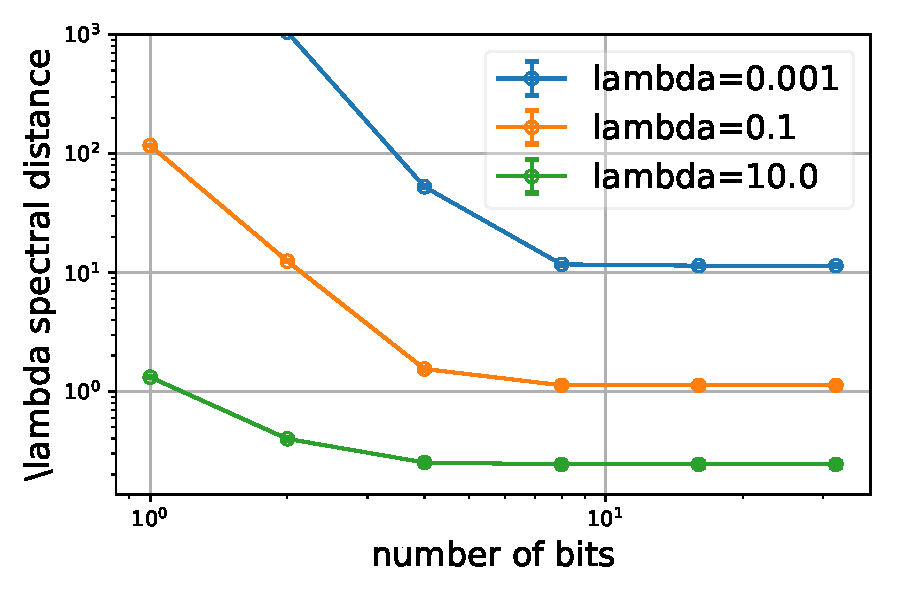
\includegraphics[width=0.3\linewidth]{figures/theory_fixed_n_feat.pdf} &
		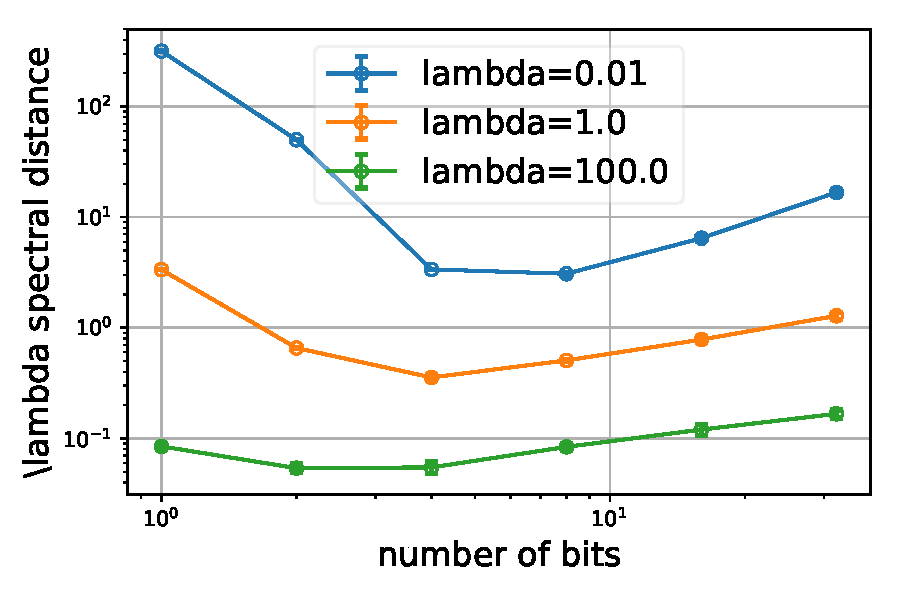
\includegraphics[width=0.3\linewidth]{figures/theory_fixed_memory.pdf} &
		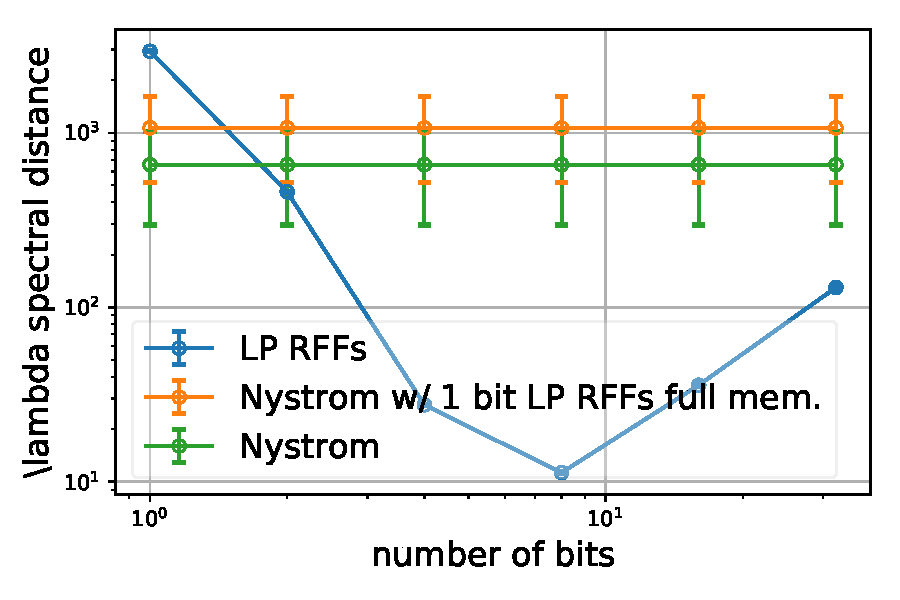
\includegraphics[width=0.3\linewidth]{figures/theory_fixed_memory_generous_mem_to_nystrom_lamb_0001.pdf} 
	\end{tabular}
	\caption{Empirical validation of Theorem \ref{thm2}.  We demonstrate that the optimal precision, in terms of lowest relative spectral distance per bit, depends on the value of $\lambda$.}
	\label{fig:theo_validation}
\end{figure}

\subsection{Systems considerations}
While the majority of this paper focuses on analyzing the statistical and empirical properties of LP-RFFs, it is also important to consider how a training algorithm using these features could be implemented. While in theory one could perform a matrix multiplication between a mini-batch of low-precision features and a full-precision model, this type of operation is not generally available on real systems. As a result, one would need to cast the LP-RFFs back into full-precision, in effect eliminating the computational benefit of using low-precision in the first place.  In order to avoid this, one could store the model itself in low-precision. In Section \ref{sec:halp}, we present our experimental results using a low-precision training algorithm called HALP \citep{halp18}, showing that on TIMIT, with 8 bit features and an 8 bit model, we can match the generalization performance of full-precision training on the 8 bit features.

A second technical challenge is that in the current definition of LP-RFFs, the full-precision features are calculated and then quantized to $b$ bits each. If the full-precision feature calculation is done in batch, this means that enough memory is needed in order to store all of the full-precision features in the mini-batch simultaneously. One solution is to compute the low-precision features in blocks, where we quantize the output of one block before computing the next one. This lowers the memory footprint, while still allowing us to benefit from fast matrix multiplications for each block. Another option is to use low-precision for all parts of the feature generation process (\eg, quantize, $x$, $w$, and $a$, and then compute $\cos(x^T w + a)$).  We leave this for future work.


